% !TEX TS-program = pdflatex
% !TEX encoding = UTF-8 Unicode

\documentclass{beamer}
%\documentclass[handout]{beamer}

%\setbeamertemplate{background canvas}[vertical shading][bottom=white,top=structure.fg!25]
% or whatever

\usetheme[compress]{Amsterdam}
%\setbeamertemplate{headline}{}
%\setbeamertemplate{footline}{}
%\setbeamersize{text margin left=0.5cm}
  
\usepackage[english]{babel}
\usepackage{listings}
\usepackage{geometry}
\usepackage{hyperref}

\usepackage{color}
\usepackage[T1]{fontenc}
\usepackage[utf8]{inputenc}
\usepackage{lmodern}


\usepackage{tikz}
\usetikzlibrary{shapes,arrows}

\usepackage{multicol}
\lstset{
basicstyle=\scriptsize\ttfamily,
columns=flexible,
breaklines=true,
numbers=left,
%stepsize=1,
numberstyle=\tiny,
backgroundcolor=\color[rgb]{0.85,0.90,1}
}


\begin{document}

\title[Big Data and Automated Content Analysis]{\textbf{Big Data and Automated Content Analysis} \\ Week 7 -- Thursday  \\ »Looking back and forward«}
\author[Anne Kroon]{Anne Kroon \\ ~ \\ \footnotesize{a.c.kroon@uva.nl \\@annekroon} \\}
\date{May 16, 2019}
\institute[UvA]{Afdeling Communicatiewetenschap \\Universiteit van Amsterdam}


\tikzstyle{block} = [rectangle, draw, fill=blue!20, 
text width=5em, text centered, rounded corners, minimum height=4em]
\tikzstyle{line} = [draw]
\tikzstyle{pijltje} = [draw, -latex']
\tikzstyle{cloud} = [draw, ellipse,fill=red!20, node distance=3cm,
minimum height=2em, text width=4em, text centered,]

















\begin{frame}{}
\titlepage
\end{frame}

\begin{frame}{Today}
\tableofcontents
\end{frame}




\section{Looking back}
\subsection{Putting the pieces together}
\begin{frame}[plain]{}
Looking back\\
\textbf{Putting the pieces together}
\end{frame}


\begin{frame}{First: Our epistomological underpinnings}
	Computational Social Science
\end{frame}


\begin{frame}{Computational Social Science}
	``It is an approach to social inquiry defined by (1) the use of large, complex datasets, often—though not always— measured in terabytes or petabytes; (2) the frequent involvement of “naturally occurring” social and digital media sources and other electronic databases; (3) the use of computational or algorithmic solutions to generate patterns and inferences from these data; and (4) the applicability to social theory in a variety of domains from the study of mass opinion to public health, from examinations of political events to social movements''
	
	\vskip 0.5 cm
	\tiny{Shah, D. V., Cappella, J. N., \& Neuman, W. R. (2015). Big Data, digital media, and computational social science: Possibilities and perils. T\textit{he ANNALS of the American Academy of Political and Social Science, 659}(1), 6–13. doi:10.1177/0002716215572084}
\end{frame}





\begin{frame}{Computational Social Science}
``[\ldots] the computational social sciences employ the scientific method, complementing descriptive statistics with inferential statistics that seek to identify associations and causality. In other words, they are underpinned by an epistemology wherein the aim is to produce sophisticated statistical models that explain, simulate and predict human life.''

\vskip 0.5 cm
\tiny{Kitchin, R. (2014). Big Data, new epistemologies and paradigm shifts. \textit{Big Data \& Society, 1}(1), 1–12. doi:10.1177/2053951714528481}
\end{frame}

%
%\begin{frame}{Second: Our data}
%	content...
%\end{frame}
%
%
%
%
%\begin{frame}{Third: Our techniques}
%	content...
%	\end{frame}




\begin{frame}{Steps of a CSS project}
We learned techniques for:
\begin{itemize}
	\item retrieving data
	\item processing data
	\item analyzing data
	\item visualising data
\end{itemize}

\end{frame}

\begin{frame}[plain]
\begin{tikzpicture}[node distance = 3cm, auto]
\node [cloud] (retrieve) {retrieve};
\node [cloud, right of=retrieve] (process) {process and/or enrich};
\node [cloud, right of=process] (analyze) {analyze\\ explain\\ predict};
\node [cloud, right of=analyze] (visualize) {communi-cate};


\path [pijltje] (retrieve)--(process);
\path [pijltje] (process)--(analyze);
\path [pijltje] (analyze)--(visualize);


\node [block, below of = retrieve] (retrievetech) {files\\ APIs\\ scraping};
\node [block, below of= process] (processtech) {NLP\\ sentiment\\ LDA\\ SML};
\node [block, below of=analyze] (analyzetech) {group comparisons; statistical tests and models};
\node [block, below of=visualize] (visualizetech) {visualizations and summary tables};


\path [pijltje] (retrievetech)--(processtech);
\path [pijltje] (processtech)--(analyzetech);
\path [pijltje] (analyzetech)--(visualizetech);


\node [block, below of = retrievetech, fill=green!20] (retrievepython) {glob\\ json \& csv\\ requests\\ lxml\\ \ldots};

\node [block, below of = processtech, fill=green!20] (processpython) {nltk\\ pattern \\ vader \\ gensim\\ scikit-learn \ldots};

\node [block, below of = analyzetech, fill=green!20] (analyzepython) {numpy/scipy\\ pandas\\ statsmodels\\ \ldots};

\node [block, below of = visualizetech, fill=green!20] (visualizepython) {pandas\\ matplotlib\\ seaborn\\ pyldavis\\ \ldots};





\path [line, dashed] (retrieve)--(retrievetech);
\path [line, dashed] (process)--(processtech);
\path [line, dashed] (analyze)--(analyzetech);
\path [line, dashed] (visualize)--(visualizetech);



\path [line, dashed] (retrievetech)--(retrievepython);
\path [line, dashed] (processtech)--(processpython);
\path [line, dashed] (analyzetech)--(analyzepython);
\path [line, dashed] (visualizetech)--(visualizepython);
\end{tikzpicture}
\end{frame}

\subsection{A good workflow}
\begin{frame}
	A good workflow
\end{frame}


\begin{frame}{The big picture}
\begin{block}{Start with pen and paper}
\begin{enumerate}[<+->]
	\item Draw the Big Picture
	\item Then work out what components you need
\end{enumerate}
\end{block}
\end{frame}


\begin{frame}{Develop components separately}
	\begin{block}{One script for downloading the data, one script for analyzing}
		\begin{itemize}[<+->]
			\item Avoids waste of resources (e.g., unnecessary downloading multiple times)
			\item Makes it easier to re-use your code or apply it to other data
		\end{itemize}
	\end{block}
\pause
\begin{block}{Start small, then scale up}
	\begin{itemize}[<+->]
		\item Take your plan (see above) and solve \textit{one} problem at a time (e.g., parsing a review page; or getting the URLs of all review pages)
		\item (for instance, by using functions [next slides])
	\end{itemize}
\end{block}

\end{frame}	


\begin{frame}{Develop components separately}
	\begin{block}{If you copy-paste code, you are doing something wrong}
		\begin{itemize}[<+->]
			\item Write loops!
			\item If something takes more than a couple of lines, write a function!
		\end{itemize}
	\end{block}
\end{frame}

\begin{frame}[plain, fragile]
Copy-paste approach\\ (ugly, error-prone, hard to scale up)
\begin{lstlisting}
allreviews = []

response = requests.get('http://xxxxx')
tree =  fromstring(response.text)
reviewelements = tree.xpath('//div[@class="review"]')
reviews = [e.text for e in reviewelements]
allreviews.extend(reviews)

response = requests.get('http://yyyyy')
tree =  fromstring(response.text)
reviewelements = tree.xpath('//div[@class="review"]')
reviews = [e.text for e in reviewelements]
allreviews.extend(reviews)
\end{lstlisting}
\end{frame}


\begin{frame}[plain, fragile]
Better: for-loop\\ (easier to read, less error-prone, easier to scale up (e.g., more URLs, read URLs from a file or existing list)))
\begin{lstlisting}
allreviews = []

urls = ['http://xxxxx', 'http://yyyyy']

for url in urls:
    response = requests.get(url)
    tree =  fromstring(response.text)
    reviewelements = tree.xpath('//div[@class="review"]')
    reviews = [e.text for e in reviewelements]
    allreviews.extend(reviews)
\end{lstlisting}
\end{frame}




\begin{frame}[plain, fragile]
Even better: for-loop with functions\\ (main loop is easier to read, function can be re-used in multiple contexts)
\begin{lstlisting}
def getreviews(url):
    response = requests.get(url)
    tree =  fromstring(response.text)
    reviewelements = tree.xpath('//div[@class="review"]')
    return [e.text for e in reviewelements]


urls = ['http://xxxxx', 'http://yyyyy']

allreviews = []

for url in urls:
    allreviews.extend(getreviews(url))
\end{lstlisting}
\end{frame}


\begin{frame}{Scaling up}
	Until now, we did not look too much into aspects like code style, re-usability, scalability
	\begin{itemize}
		\item Use functions and classes (Appendix D.3) to make code more readable and re-usable
		\item Avoid re-calculating values
		\item Think about how to minimize memory usage (e.g., Generators, Appendix D.2)
		\item Do not hard-code values, file names, etc., but take them as arguments
	\end{itemize}	
\end{frame}




\begin{frame}{Make it robust}
You cannot foresee every possible problem.\\
Most important: Make sure your program does not fail and loose all data just because something goes wrong at case 997/1000.
	\begin{itemize}
		\item Use \texttt{try/except} to explicitly tell the program how to handle errors
		\item Write data to files (or database) in between
		\item Use \texttt{assert len(x) == len(y}) for sanity checks
	\end{itemize}	
\end{frame}


%
%
%\begin{frame}{Replicability}
%	\begin{block}{ddd}
%		\begin{enumerate}[<+->]
%			\item egjkrjhh
%		\end{enumerate}
%	\end{block}
%\end{frame}






%{\setbeamercolor{background canvas}{bg=black}
%\begin{frame}[plain]
%\makebox[\linewidth]{
%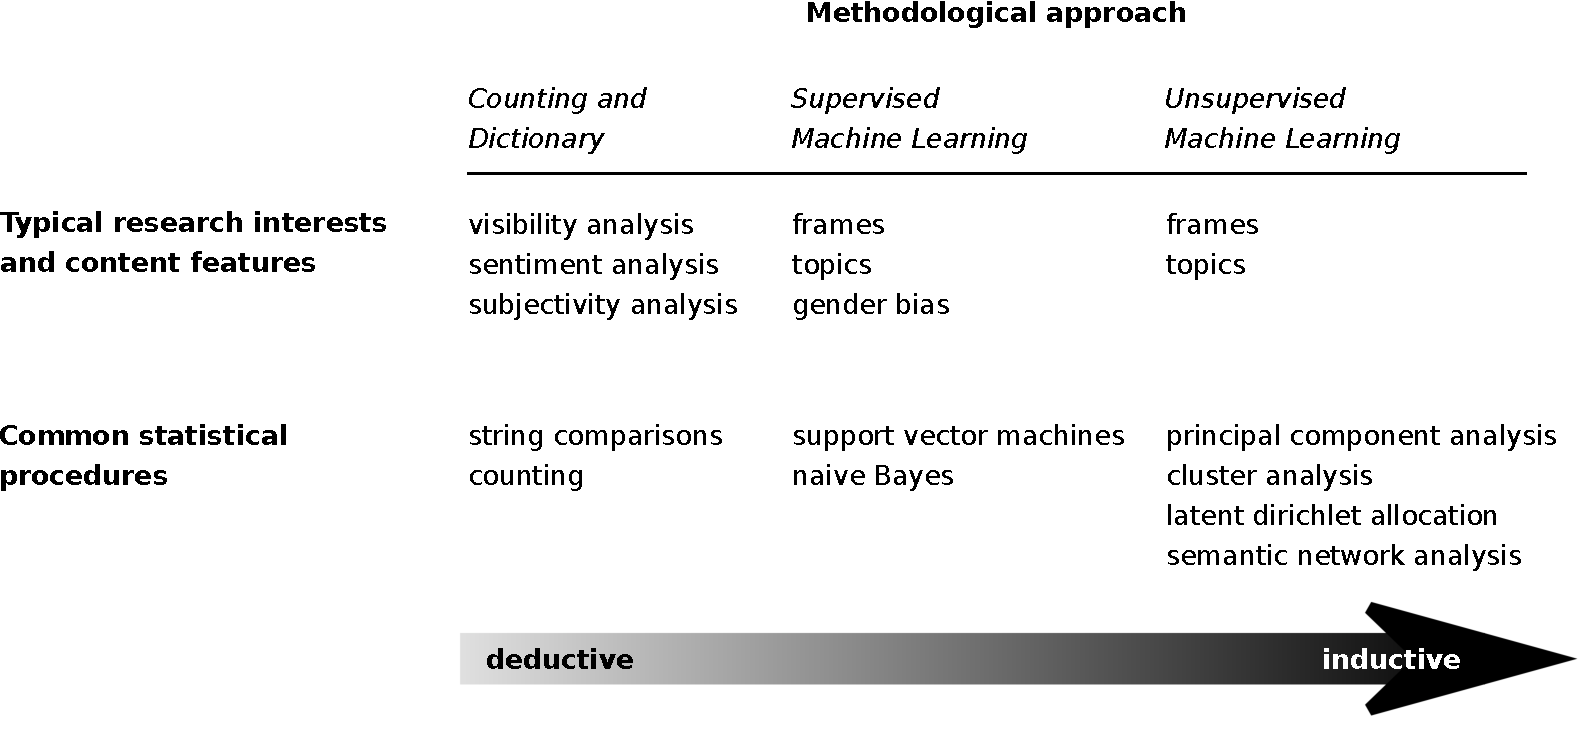
\includegraphics[width=\paperwidth,height=\paperheight,keepaspectratio]{../../pictures//boumanstrilling2016}}
%\end{frame}
%}



%
%\begin{frame}{Some terminology }
%	\begin{columns}[t]
%		\column{.5\textwidth}
%		
%		\begin{block}<1-4>{Supervised machine learning}
%			You have a dataset with both predictor and outcome (independent and dependent variables; features and labels) --- a \emph{labeled} dataset.
%			\onslide<2>{
%				\footnotesize{Think of regression: You measured \texttt{x1}, \texttt{x2}, \texttt{x3} and you want to predict \texttt{y}, which you also measured}}
%		\end{block}
%		
%		\column{.5\textwidth}
%		
%		\begin{block}<3->{Unsupervised machine learning}
%			You have no labels. \onslide<4>{(\footnotesize{You did not measure \texttt{y})}}\\
%			\onslide<5>{\textbf{Again, you already know some techniques to find out how \texttt{x1}, \texttt{x2},\ldots \texttt{x\_i} co-occur from other courses:} \begin{itemize}
%					\item Principal Component Analysis (PCA)
%					\item Cluster analysis
%					\item \ldots
%				\end{itemize}
%			}
%		\end{block}
%		
%	\end{columns}
%	
%\end{frame}
%
%



\section{Looking forward}
\subsection{Techniqes we did not cover}
\begin{frame}[plain]{}
Looking forward\\
\textbf{What other possibilities do exist for each step?}
\end{frame}


\begin{frame}[plain]
	\begin{tikzpicture}[node distance = 3cm, auto]
	\node [cloud] (retrieve) {retrieve};
	\node [cloud, right of=retrieve] (process) {process and/or enrich};
	\node [cloud, right of=process] (analyze) {analyze\\ explain\\ predict};
	\node [cloud, right of=analyze] (visualize) {communi-cate};
	
	
	\path [pijltje] (retrieve)--(process);
	\path [pijltje] (process)--(analyze);
	\path [pijltje] (analyze)--(visualize);
	
	
	\node [block, below of = retrieve] (retrievetech) {?};
	\node [block, below of= process] (processtech) {?};
	\node [block, below of=analyze] (analyzetech) {?};
	\node [block, below of=visualize] (visualizetech) {?};
	
	
	
	\path [pijltje] (retrievetech)--(processtech);
	\path [pijltje] (processtech)--(analyzetech);
	\path [pijltje] (analyzetech)--(visualizetech);
	
	
	\node [block, below of = retrievetech, fill=green!20] (retrievepython) {?};
	
	\node [block, below of = processtech, fill=green!20] (processpython) {?};
	
	\node [block, below of = analyzetech, fill=green!20] (analyzepython) {?};
	
	\node [block, below of = visualizetech, fill=green!20] (visualizepython) {?};
	
	
	
	
	
	\path [line, dashed] (retrieve)--(retrievetech);
	\path [line, dashed] (process)--(processtech);
	\path [line, dashed] (analyze)--(analyzetech);
	\path [line, dashed] (visualize)--(visualizetech);
	
	
	
	\path [line, dashed] (retrievetech)--(retrievepython);
	\path [line, dashed] (processtech)--(processpython);
	\path [line, dashed] (analyzetech)--(analyzepython);
	\path [line, dashed] (visualizetech)--(visualizepython);
	\end{tikzpicture}
\end{frame}



\begin{frame}{Retrieve}
	\begin{block}{Webscraping with Selenium}
	\begin{itemize}
		\item 	If content is dynamically loaded (e.g., with JavaScript), our approach doesn't work (because we don't have a browser).
		\item 	Solution: Have Python literally open a browser and literally click on things
		\item $\Rightarrow$ Appendix E
	\end{itemize}
	\end{block}
\end{frame}



\begin{frame}{Retrieve}
	\begin{block}{Use of databases}
	We did not discuss how to actually store the data
	\begin{itemize}
		\item We basically stored our data in files (often, one CSV or JSON file)
		\item But that's not very efficient if we have large datasets; especially if we want to select subsets later on
		\item SQL-databases to store tables (e.g., MySQL)
		\item NoSQL-databases to store less structured data (e.g., JSON with unknown keys) (e.g., MongoDB, ElasticSearch)
		\item $\Rightarrow$ \tiny{Günther, E., Trilling, D., \& Van de Velde, R.N. (2018). But how do we store it? (Big) data architecture in the social-scientific research process. In:\textit{ Stuetzer, C.M., Welker, M., \& Egger, M. (eds.): Computational Social Science in the Age of Big Data. Concepts, Methodologies, Tools, and Applications}. Cologne, Germany: Herbert von Halem.}
	\end{itemize}
	\end{block}
\end{frame}


\begin{frame}{Storing data}
	\makebox[\linewidth]{
		\includegraphics[width=\paperwidth,height=\paperheight,keepaspectratio]{../../pictures/guenteretal_fig1}}
\end{frame}


\begin{frame}{From retrieved data to enriched data}
	\makebox[\linewidth]{
		\includegraphics[width=\paperwidth,height=\paperheight,keepaspectratio]{../../pictures/guentheretal_fig3}}
\end{frame}




\begin{frame}{Process and/or enrich}
	\begin{block}{Word embeddings}
	We did not really consider the \emph{meaning} of words
		\begin{itemize}
		\item Word embeddings can be trained on large corpora (e.g., whole wikipedia or a couple of years of newspaper coverage) 
		\item The trained model allows you to calculate with words (hence, word vectors): $king-man+woman = ?$ 
		\item You can find out whether documents are similar \emph{even if they do not use the same words} (Word Mover Distance)
		\item $\Rightarrow$ word2vec (in gensim!), glove
		\end{itemize}
	\end{block}
\end{frame}

{\setbeamercolor{background canvas}{bg=lightgray}
	\begin{frame}[plain]
	\makebox[\linewidth]{
		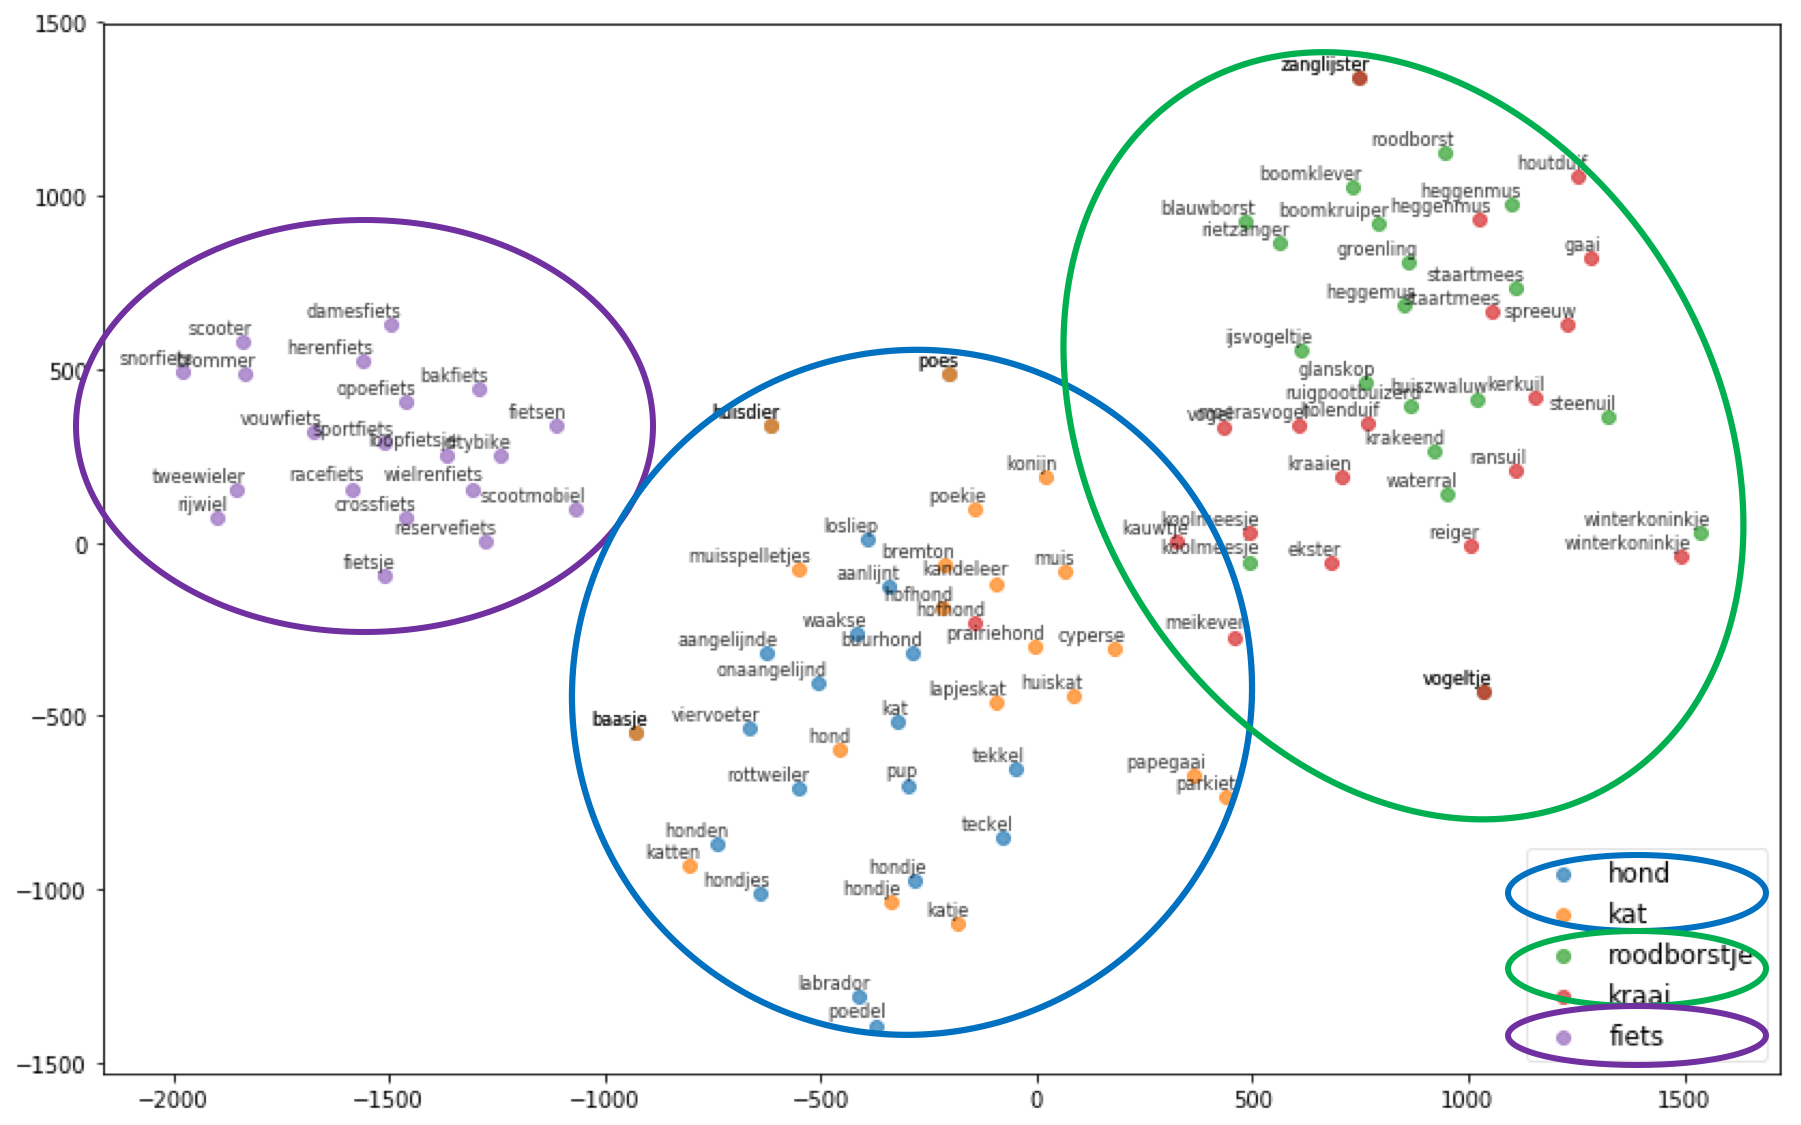
\includegraphics[width=\paperwidth,height=\paperheight,keepaspectratio]{../../pictures/visual.png}}
\end{frame}

}


\begin{frame}{Process and/or enrich}
	\begin{block}{Advanced NLP}
		We did a lot of BOW (and some POS-tagging), but we can get more
		\begin{itemize}
			\item Named Entity Recognition (NER) to get names of people, organizations, \ldots
			\item Dependency Parsing to find out exact relationships
			$\Rightarrow$ nltk, Stanford, FROG, Spacy
		\end{itemize}
	\end{block}
\end{frame}


{\setbeamercolor{background canvas}{bg=lightgray}
\begin{frame}[plain]
\makebox[\linewidth]{
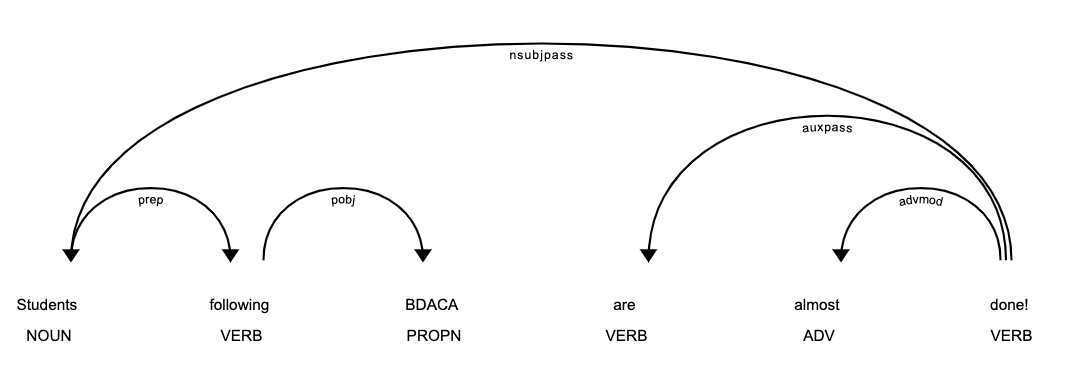
\includegraphics[width=\paperwidth,height=\paperheight,keepaspectratio]{../../pictures/dependencies_spacy.png}}
PREP: Prepositional modifier \\
NSUBJPASS: Nominal subject (passive) \\
AUXPASS: Auxiliary (passive) \\
\end{frame}

}



\begin{frame}{Analyze/explain/predict}
	\begin{block}{More advanced modelling}
We only did some basic statistical tests
		\begin{itemize}
			\item Especially with social media data, we often have time series (VAR models etc.)
		%	\item There are more advanced regression techniques and dimension-reduction techniques tailored to data that are, e.g., large-scale, sparse, have a lot of features, \ldots
		\item $\Rightarrow$ scikit-learn, statsmodels
		\end{itemize}
	\end{block}
\end{frame}


\section[Advanced ACA]{Advanced Types of Automated Content Analysis}
\begin{frame}{}
Recap: Types of Automated Content Analysis
\end{frame}

\subsection*{Top-down vs. bottom-up}

%{\setbeamercolor{background canvas}{bg=black}
\begin{frame}[plain]
\makebox[\linewidth]{
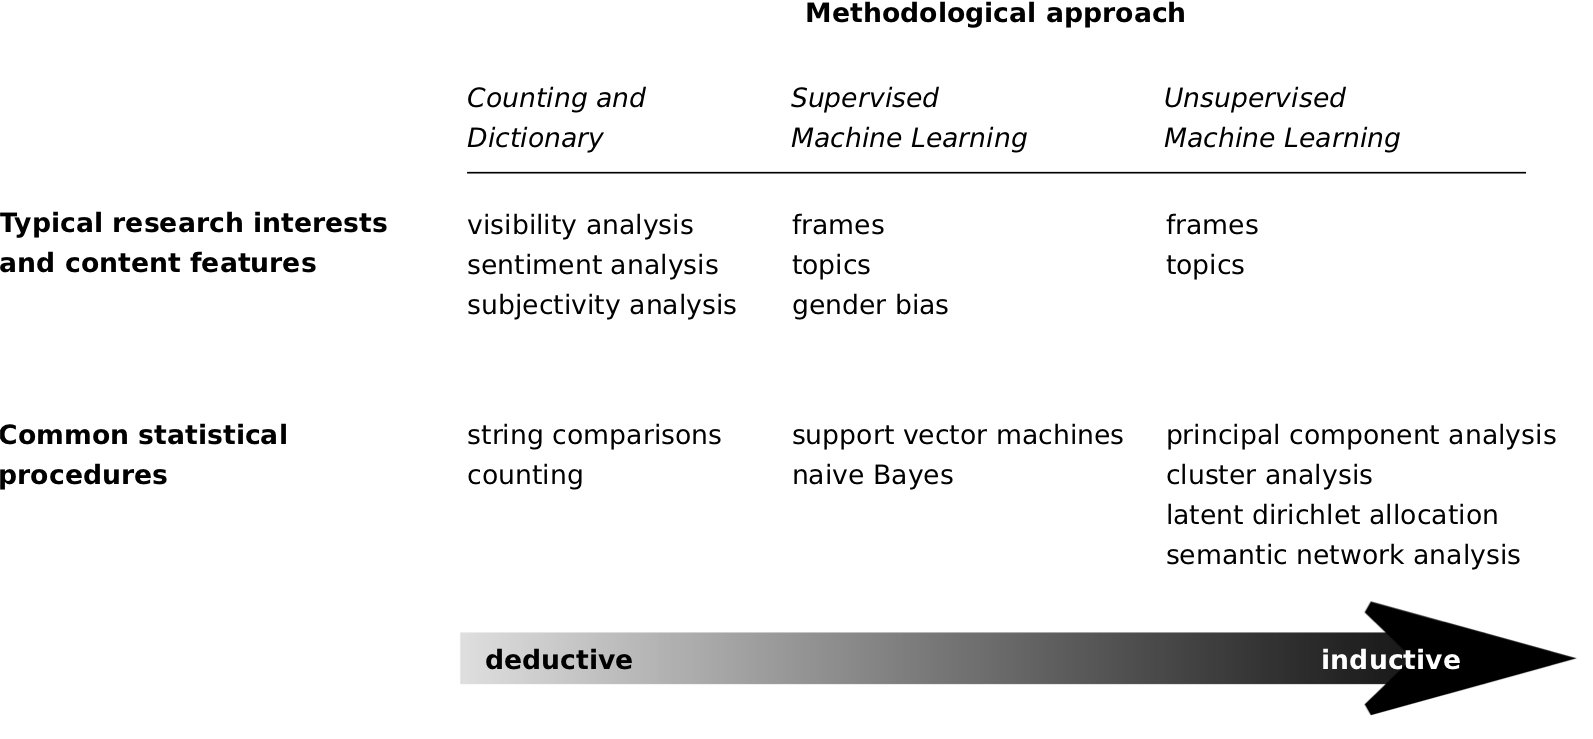
\includegraphics[width=\paperwidth,height=\paperheight,keepaspectratio]{../../pictures//boumanstrilling2016_.png}}
\end{frame}
%}


\begin{frame}{Some terminology }
\begin{columns}[t]
\column{.5\textwidth}

\begin{block}<1-4>{Supervised machine learning}
You have a dataset with both predictor and outcome (independent and dependent variables; features and labels) --- a \emph{labeled} dataset.
\onslide<2>{
	\footnotesize{Think of regression: You measured \texttt{x1}, \texttt{x2}, \texttt{x3} and you want to predict \texttt{y}, which you also measured}}
\end{block}

\column{.5\textwidth}

\begin{block}<3->{Unsupervised machine learning}
You have no labels. \onslide<4>{(\footnotesize{You did not measure \texttt{y})}}\\
\onslide<5>{\textbf{Again, you already know some techniques to find out how \texttt{x1}, \texttt{x2},\ldots \texttt{x\_i} co-occur from other courses:} \begin{itemize}
		\item Principal Component Analysis (PCA)
		\item Cluster analysis
		\item \ldots
	\end{itemize}
}
\end{block}

\end{columns}

\end{frame}




\section{Unsupervised ML}
\begin{frame}[plain]
inductive and bottom-up:\\ \textbf{unsupervised machine learning}\\
\vspace{1cm}\hspace{1cm} \onslide<2> \footnotesize{(something you aready did in your Bachelor -- no kidding.)}
\end{frame}



\subsection{PCA}




\begin{frame}{Principal Component Analysis? How does \emph{that} fit in here?}
\onslide<2>{In fact, PCA is used everywhere, even in image compression}

\begin{block}<3->{PCA in ACA}
\begin{itemize}
\item Find out what word cooccur (inductive frame analysis)
\item Basically, transform each document in a vector of word frequencies and do a PCA
\end{itemize}
\end{block}
%\onslide<4>{\textbf{But we'll look at the state of the art instead: Latent Dirichlet Allication (LDA)}}
\end{frame}

\begin{frame}[fragile]{A so-called term-document-matrix}
\begin{lstlisting}
w1,w2,w3,w4,w5,w6 ...
text1, 2, 0, 0, 1, 2, 3 ...
text2, 0, 0, 1, 2, 3, 4 ...
text3, 9, 0, 1, 1, 0, 0 ...
...
\end{lstlisting}
\vspace{1cm}
\onslide<2->{These can be simple counts, but also more advanced metrics, like tf-idf scores (where you weigh the frequency by the number of documents in which it occurs), cosine distances, etc.}
\vspace{5mm}
\onslide<3> $\mbox{W}_{i,j} =  \mbox{tf}_{i,j}  \cdot \log ( \frac{N}{\mbox{df}_i } )

\end{frame}


\begin{frame}{PCA: implications and problems}
\begin{itemize}
\item given a term-document matrix, easy to do with any tool
\item probably extremely skewed distributions
\item some problematic assumptions: does the goal of PCA, to find a solution in which one word loads on \emph{one} component match real life, where a word can belong to several topics or frames?
\end{itemize}
\end{frame}



\subsection{LDA}


\begin{frame}{}
Enter \textbf{topic modeling with Latent Dirichlet Allocation (LDA)}
\end{frame}



\begin{frame}{LDA, what's that?}
\begin{block}{No mathematical details here, but the general idea}
\begin{itemize}
\item There are $k$ topics, $T_1$\ldots$T_k$
\item Each document $D_i$ consists of a mixture of these topics, e.g.$80\% T_1, 15\% T_2, 0\% T_3, \ldots 5\% T_k $
\item On the next level, each topic consists of a specific probability distribution of words
\item Thus, based on the frequencies of words in $D_i$, one can infer its distribution of topics
\item Note that LDA (like PCA) is a Bag-of-Words (BOW) approach
\end{itemize}
\end{block}

\end{frame}




\begin{frame}[fragile]{Doing a LDA in Python}
You can use gensim ({\v R}eh{\r u}{\v r}ek \& Sojka, 2010) for this.

Let us assume you have a list of lists of words (!) called \texttt{texts}:

\begin{lstlisting}
articles=['The tax deficit is higher than expected. This said xxx ...', 'Germany won the World Cup. After a']
texts=[art.split() for art in articles]
\end{lstlisting}
which looks like this:
\begin{lstlisting}
[['The', 'tax', 'deficit', 'is', 'higher', 'than', 'expected.', 'This', 'said', 'xxx', '...'], ['Germany', 'won', 'the', 'World', 'Cup.', 'After', 'a']]
\end{lstlisting}

\tiny{{\v R}eh{\r u}{\v r}ek, R., \& Sojka, P. (2010). Software framework for topic modelling with large corpora. \emph{Proceedings of the LREC 2010 Workshop on New Challenges for NLP Frameworks}, pp. 45–50. Valletta, Malta: ELRA. }

\end{frame}




\begin{frame}[plain,fragile]
\begin{lstlisting}
from gensim import corpora, models

NTOPICS = 100
LDAOUTPUTFILE="topicscores.tsv"

# Create a BOW represenation of the texts
id2word = corpora.Dictionary(texts)
mm =[id2word.doc2bow(text) for text in texts]

# Train the LDA models.
mylda = models.ldamodel.LdaModel(corpus=mm, id2word=id2word, num_topics=NTOPICS, alpha="auto")

# Print the topics.
for top in mylda.print_topics(num_topics=NTOPICS, num_words=5):
print ("\n",top)

print ("\nFor further analysis, a dataset with the topic score for each document is saved to",LDAOUTPUTFILE)

scoresperdoc=mylda.inference(mm)

with open(LDAOUTPUTFILE,"w",encoding="utf-8") as fo:
for row in scoresperdoc[0]:
fo.write("\t".join(["{:0.3f}".format(score) for score in row]))
fo.write("\n")
\end{lstlisting}

\end{frame}


\begin{frame}[fragile]{Output: Topics (below) \& topic scores (next slide)}
\begin{lstlisting}
0.069*fusie + 0.058*brussel + 0.045*europesecommissie + 0.036*europese + 0.023*overname
0.109*bank + 0.066*britse + 0.041*regering + 0.035*financien + 0.033*minister
0.114*nederlandse + 0.106*nederland + 0.070*bedrijven + 0.042*rusland + 0.038*russische
0.093*nederlandsespoorwegen + 0.074*den + 0.036*jaar + 0.029*onderzoek + 0.027*raad
0.099*banen + 0.045*jaar + 0.045*productie + 0.036*ton + 0.029*aantal
0.041*grote + 0.038*bedrijven + 0.027*ondernemers + 0.023*goed + 0.015*jaar
0.108*werknemers + 0.037*jongeren + 0.035*werkgevers + 0.029*jaar + 0.025*werk
0.171*bank + 0.122* + 0.041*klanten + 0.035*verzekeraar + 0.028*euro
0.162*banken + 0.055*bank + 0.039*centrale + 0.027*leningen + 0.024*financiele
0.052*post + 0.042*media + 0.038*nieuwe + 0.034*netwerk + 0.025*personeel
...
\end{lstlisting}
\end{frame}


\begin{frame}[plain]
\makebox[\linewidth]{
\includegraphics[width=\paperwidth,height=\paperheight,keepaspectratio]{../../pictures/topicscores}}
\end{frame}




\begin{frame}[fragile]{Visualization with pyldavis}
\begin{lstlisting}
import pyLDAvis
import pyLDAvis.gensim
# first estiate gensim model, then:
vis_data = pyLDAvis.gensim.prepare(mylda,mm,id2word)
pyLDAvis.display(vis_data)
\end{lstlisting}
\makebox[\linewidth]{
\includegraphics[width=\paperwidth,height=.5\paperheight,keepaspectratio]{../../pictures/pyldavis}}
\end{frame}







\section[Supervised ML]{Supervised Machine Learning}

\begin{frame}[plain]
predefined categories, but no predefined rules:\\ \textbf{supervised machine learning}\\
\vspace{1cm}\hspace{1cm} \onslide<2> \footnotesize{(something you aready did in your Bachelor -- no kidding.)}
\end{frame}








\begin{frame}{Recap: supervised vs. unsupervised}
\begin{columns}[t]

\column{.5\textwidth}

\begin{block}{Unsupervised}<1->
\begin{itemize}
\item No manually coded data
\item We want to identify patterns or to make groups of most similar cases
%\item Per case, we want to know to which group it belongs
\end{itemize}
\end{block}
{\footnotesize{
\onslide<2->{Example: We have a dataset of Facebook-massages on an organizations' page. We use clustering to group them and later interpret these clusters (e.g., as complaints, questions, praise, \ldots)}
}}

\column{.5\textwidth}
\begin{block}{Supervised}<3->
\begin{itemize}
\item We code a small dataset by hand and use it to ``train'' a machine
\item The machine codes the rest 
\end{itemize}
\end{block}

{\footnotesize{
\onslide<4->{Example: %We use a hand-coded CSV table with two columns (tweet and gender of the sender) as training dataset and then predict for a different dataset per tweet if it was sent by a man or a woman.
We have 2,000 of these messages grouped into such categories by human coders. We then use this data to group all remaining messages as well.
}
}}

\end{columns}
\end{frame}





\subsection{You have done it before!}
\begin{frame}{You have done it before!}
\begin{block}{Regression}<2->
\begin{enumerate}
\item<3-> Based on your data, you estimate some regression equation 	$y_i = \alpha + \beta_1 x_{i1} + \cdots + \beta_p x_{ip} + \varepsilon_i$
\item<4-> Even if you have some \emph{new unseen data}, you can estimate your expected outcome $\hat{y}$!
\item<5-> Example: You estimated a regression equation where $y$ is newspaper reading in days/week: $y = -.8 + .4 \times man + .08 \times age$
\item<6-> You could now calculate $\hat{y}$ for a man of 20 years and a woman of 40 years -- \emph{even if no such person exists in your dataset}: \\
$\hat{y}_{man20} = -.8 + .4 \times 1 + .08 \times 20 = 1.2$ \\
$\hat{y}_{woman40} = -.8 + .4 \times 0 + .08 \times 40 = 2.4$
\end{enumerate}
\end{block}	

\end{frame}


\begin{frame}{}
\huge{This is\\ Supervised Machine Learning!}
\end{frame}

\begin{frame}{\ldots but\ldots}
\begin{itemize}
\item<1-> We will only use \emph{half} {\tiny{(or another fraction)}} of our data to estimate the model, so that we can use the other half to check if our predictions match the manual coding (``labeled data'',``annotated data'' in SML-lingo)
\begin{itemize}
\item<2->e.g., 2000 labeled cases, 1000 for training, 1000 for testing --- if successful, run on 100,000 unlabeled cases
\end{itemize}
\item<3-> We use many more independent variables (``features'')
\item<4-> Typically, IVs are word frequencies (often weighted, e.g. tf$\times$idf) ($\Rightarrow$BOW-representation)
\end{itemize}
\end{frame}


\subsection{Applications}

\begin{frame}{Applications}
\begin{block}<2->{In other fields}
\emph{A lot} of different applications
\begin{itemize}
\item  This principle can be applied to many fields and disciplines -- for example, it is possible to teach a computer to indicate if a tumor is present or not on X-rays of people's brains
\item from recognizing hand-written characters to recommendation systems
\item  Supervised Machine learning does not care about what the features mean, so instead of texts we can also classify pictures
%\item  Based on a pre-coded training set, the computer compares images sorted into two (or more) groups
\end{itemize}
\end{block}

\begin{block}<3>{In our field}
It starts to get popular to measure latent variables
\begin{itemize}
\item frames / topics
\end{itemize}
\end{block}
\end{frame}



\begin{frame}{SML to code frames and topics}
\begin{block}{Some work by Burscher and colleagues}
\begin{itemize}
\item Humans can code generic frames (human-interest, economic, \ldots)
\item Humans can code topics from a pre-defined list 
\item<2->\textbf{But it is very hard to formulate an explicit rule} \\(as in: code as 'Human Interest' if regular expression R is matched)
\end{itemize}
\onslide<3>$\Rightarrow$ This is where you need supervised machine learning!
\end{block}
\tiny{Burscher, B., Odijk, D., Vliegenthart, R., De Rijke, M., \& De Vreese, C. H. (2014). Teaching the computer to code frames in news: Comparing two supervised machine learning approaches to frame analysis. \emph{Communication Methods and Measures, 8}(3), 190–206. doi:10.1080/19312458.2014.937527
\\
Burscher, B., Vliegenthart, R., \& De Vreese, C. H. (2015). Using supervised machine learning to code policy issues: Can classifiers generalize across contexts? \emph{Annals of the American Academy of Political and Social Science, 659}(1), 122–131.
}

\end{frame}





{\setbeamercolor{background canvas}{bg=black}
\begin{frame}[plain]
\makebox[\linewidth]{
\includegraphics[width=\paperwidth,height=\paperheight,keepaspectratio]{../../pictures/burscher2014}}
\end{frame}

\begin{frame}[plain]
\makebox[\linewidth]{
\includegraphics[width=\paperwidth,height=\paperheight,keepaspectratio]{../../pictures/burscher2015-a}}
\end{frame}

\begin{frame}[plain]
\makebox[\linewidth]{
\includegraphics[width=\paperwidth,height=\paperheight,keepaspectratio]{../../pictures/burscher2015-b}}
\end{frame}
}

\begin{frame}[plain]
\begin{columns}[]
\column{.5\textwidth}

{\tiny{http://commons.wikimedia.org/wiki/File:Precisionrecall.svg}}
\makebox[\linewidth]{
\includegraphics[width=\paperwidth,height=\paperheight,keepaspectratio]{../../pictures/precisionrecall.png}}

\column{.5\textwidth}
\begin{block}{Some measures of accuracy}
\begin{itemize}
\item Precision
\item Recall
\item $\text{F1}=2\cdot \frac{\text{precision}\cdot \text{recall}}{\text{precision}+\text{recall}}$%
\item AUC (Area under curve)
$[0,1]$, $0.5=$ random guessing
\end{itemize}
\end{block}


\end{columns}

\end{frame}





\begin{frame}{What does this mean for our research?}
\begin{block}<2>{It we have 2,000 documents with manually coded frames and topics\ldots}
\begin{itemize}
\item we can use them to train a SML classifier
\item which can code an unlimited number of new documents
\item with an acceptable accuracy
\end{itemize}
\end{block}
\onslide<2>{
\tiny{Some easier tasks even need only 500 training documents, see Hopkins, D. J., \& King, G. (2010). A method of automated nonparametric content analysis for social science. \emph{American Journal of Political Science, 54}(1), 229–247.}} 
\end{frame}



\subsection{An implementation}

\begin{frame}[fragile]{An implementation}
Let's say we have a list of tuples with movie reviews and their rating:
\begin{lstlisting}
reviews=[("This is a great movie",1),("Bad movie",-1), ... ...]
\end{lstlisting}
And a second list with an identical structure:
\begin{lstlisting}
test=[("Not that good",-1),("Nice film",1), ... ...]
\end{lstlisting}
Both are drawn from the same population, it is pure chance whether a specific review is on the one list or the other.\\
\tiny{Based on an example from \url{http://blog.dataquest.io/blog/naive-bayes-movies/}}
\end{frame}


\begin{frame}[fragile]{Training a A Naïve Bayes Classifier}
\begin{lstlisting}
from sklearn.naive_bayes import MultinomialNB
from sklearn.feature_extraction.text import CountVectorizer
from sklearn import metrics

# This is just an efficient way of computing word counts
vectorizer = CountVectorizer(stop_words='english')
train_features = vectorizer.fit_transform([r[0] for r in reviews])
test_features = vectorizer.transform([r[0] for r in test])

# Fit a naive bayes model to the training data.
nb = MultinomialNB()
nb.fit(train_features, [r[1] for r in reviews])

# Now we can use the model to predict classifications for our test features.
predictions = nb.predict(test_features)
actual=[r[1] for r in test]

# Compute the error.
fpr, tpr, thresholds = metrics.roc_curve(actual, predictions, pos_label=1)
print("Multinomal naive bayes : {0}".format(metrics.auc(fpr, tpr)))

\end{lstlisting}
\end{frame}
%
%\begin{frame}{TODO}
%TODO\\
%andere vectorizer (TFIDF)\\
%verschillen classifiers\\
%andere output (metrics summary)
%\\
%waarom is dit hier een MULTINOMIAL NB
%\\
%scikit-learn installeren\\ 
%opdracht bedenken: classifiers vergelijken
%\end{frame}



\begin{frame}[fragile]{Playing around with new data}
\begin{lstlisting}
newdata=vectorizer.transform(["What a crappy movie! It sucks!", "This is awsome. I liked this movie a lot, fantastic actors","I would not recomment it to anyone.", "Enjoyed it a lot"])
predictions = nb.predict(newdata)
print(predictions)
\end{lstlisting}
This returns, as you would expect and hope:
\begin{lstlisting} 
[-1  1 -1  1]
\end{lstlisting}


\end{frame}




\begin{frame}{But we can do even better}
We can use different vectorizers and different classifiers.
\end{frame}

\begin{frame}{Different vectorizers}
\begin{itemize}
\item CountVectorizer (=simple word counts)
\item TfidfVectorizer (word counts (``term frequency'') weighted by number of documents in which the word occurs at all (``inverse document frequency''))
\item additional options: stopwords, thresholds for minimum frequencies etc.
\end{itemize}
\end{frame}

\begin{frame}{Different classifiers}
\begin{itemize}
\item Naïve Bayes
\item Logistic Regression
\item Support Vector Machine (SVM)
\item \ldots
\end{itemize}
Typical approach: Find out which setup performs best (see example source code in the book).
\end{frame}














\section{Final steps}

\begin{frame}{Next meeting}
\begin{block}{Monday 20 -- 5}
	Final chance for questions regarding final project (if you don't have any, you don't need to come.)
\end{block}

\begin{block}{Deadline final exam}
Hand in via filesender until Wednesday, 29–5, 23.59 \\
One .zip or .tar.gz file with
\begin{itemize}
	\item .py and/or .ipynb for code
	\item .pdf for text and figures
	\item .csv, .json, or .txt for data
	\item any additional file we need to understand or reproduce your work
\end{itemize}
\end{block}
Send to: A.C.kroon@uva.nl
\end{frame}




\end{document}

